\setcounter{chapter}{1}
\chapter{Diagrama de classes}

\begin{flushright}
	\textit{
		Dedique-se aos estudos para que eles o façam \\
		melhor para a sociedade e para si mesmo.
	} \\
	
	\textbf{Alvaro Granha Loregian}
\end{flushright}

O modelo de caso de uso é formado por diversos elementos que tem como propósito o fornecimento de uma visão do ponto de vista externo ao sistema. Essa funcionalidade, externamente observada, é fornecida por meio da colaboração entre diversos elementos, os quais são chamados de \textbf{objetos}. A colaboração entre os objetos podem ser vista em dois aspectos, os \textbf{dinâmicos} e \textbf{os estruturais estáticos}.

O aspecto dinâmico diz respeito a forma com que os objetos realizam as trocas de mensagens e as reações a eventos que ocorrem no sistemas. Já os estruturais estáticos permite visualizar como o sistema está estruturado internamente para que as funcionalidades visíveis sem produzidas \cite{bezerra2016principios}.

Assim, realizaremos uma introdução aos aspectos estruturais estáticos, demostrando os elementos que o diagrama de classes utiliza para a representar um sistema orientado a objeto. O diagrama de classe, segundo \citeonline{guedes2018uml}, é um dos mais importante e mais utilizados diagramas da UML, o qual permite a visualização da \textbf{classes} que comporão o sistemas com seus respectivos \textbf{atributos}, \textbf{métodos} e pelo relacionamento entre estes.

\section{Modelo de classes}

A medida que o sistemas é desenvolvido, o modelo de classe pode evoluir para demostrar o sistema com maior riqueza de detalhes. Assim, podemos estudar três níveis de detalhamento: \textbf{domínio}, \textbf{especificação} é \textbf{implementação} \cite{bezerra2016principios}.

\begin{itemize}
	\item \textbf{Modelo de domínio: } Nesse modelo não é levado em consideração como o sistemas será implementado mas apenas as classes que o comporão.
	\item \textbf{Modelo de especificação: } Já no modelo de especificação são adicionados detalhes específicos relacionados a solução do software.
	\item \textbf{Modelo de implementação: } Esse modelo corresponde a implementação das classes em alguma linguagem de programação. 
\end{itemize}

\section{Diagrama de classes}

O diagrama de classes, como dito anteriormente, é um dos mais importantes para o desenvolvimento de um sistema orientado a objeto. 

Como todos os diagramas da UML, o diagrama de classe é composto de elementos que, consequentemente, possuem também suas responsabilidades. Assim, veremos todos este elementos, essenciais para o modelo de domíno, e como eles interagem entre si.

Lembre-se que, o conceito relacionado a cada um já foi apresentado no Capítulo \ref{cap:cap1}.

\subsection{Classes, atributos e métodos}

Uma classe é representada por meio de uma \textbf{caixa} com, no máximo, trés compartimentos. No compartimento superior é exibido o nome da classe, o qual é o único elemento obrigatório. 

No segundo compartimento são declarados os atributos. Este, como visto no \ref{cap:cap1}, armazenam os dados que um objeto armazena. Por fim, no último compartimento são declarados os métodos. 

Assim, segundo \citeonline{bezerra2016principios}, as possíveis anotações para que possamos representar uma classe utilizando as notações UML são representadas na Figura \ref{fig:notacoes-uml-diagrama-de-classes}.

\begin{figure}[H]
	\centering
	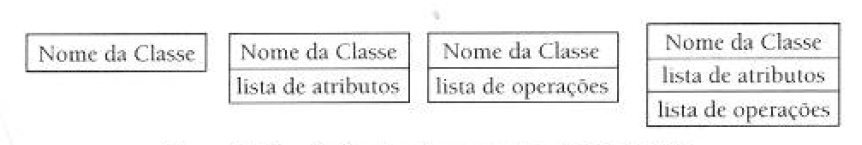
\includegraphics[scale=0.5]{imagens/notacoes-uml-classes.png}
	\caption{Possíveis notações para uma classe em UML.}
	\legend{Fonte: \cite{bezerra2016principios}}
	\label{fig:notacoes-uml-diagrama-de-classes}
\end{figure} 

Por convenção o nome das classe sempre será no singular e iniciará com letra maiúscula usando sempre o a forma de escrita conhecida como \textit{CamenCase}. Já os atributos e métodos sempre iniciarão com letra minúscula, mas também seguirão o padrão \textit{CamenCase}. Os métodos devem expressar uma ação que o objeto da classe sabe realizar. Vejamos um exemplo da classe \textbf{\textit{ContaBancaria}}.

\begin{figure}[H]
	\centering
	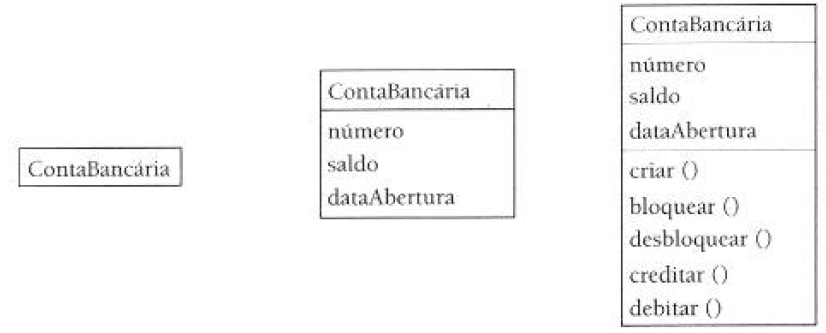
\includegraphics[scale=0.5]{imagens/exemplo-classe-conta-bancaria.png}
	\caption{Diferentes graus de detalhe para \textit{ContaBancaria}.}
	\legend{Fonte: \cite{bezerra2016principios}}
	\label{fig:exemplo-classe-conta-bancaria}
\end{figure}

\section{Exercícios de fixação}

Utilizando às notações aprendidas, identifique as possíveis classes, atributos e métodos para o problema abaixo.

\begin{enumerate}
	\item O professor \textbf{Picolo} precisa de um software para lhe ajudar a lembrar os aniversários de seus alunos. O software deve ser capaz de armazenar o nome do aluno, sua data de nascimento, seu e-mail, seu sexo e qualquer outro dado relevante. O software deve permitir o cadastro dos alunos, avisar quem faz aniversário no dia, calcular e mostrar a idade do aluno, exibir um relatório de aniversariantes no mês e outras funcionalidades que se julgar necessário.
	\item Faça o mesmo para o exercício 1 do exercício de fixação \ref{exer:001}
\end{enumerate}

\subsection{Relacionamentos}

As classes costumam ter relacionamentos entre si, com o objetivo de compartilhar informações e colaborar uma com as outras para permitir a execução dos diversos processos executados em um sistema \cite{guedes2018uml}. Assim, vermos as diversas formas de relacionamentos presentes na UML e relacionadas ao diagrama de classes.

\subsubsection{Associação}

Uma associação descreve um vínculo que ocorre normalmente entre duas classes. Esse ligação da-se o nome de \textbf{associação binária}. Contudo, há casos que a classe pode se associar a si mesmo, dando origem a um tipo de associação \textbf{chamada de unária}, ou associar-se a outras classes, a qual é chamada de \textbf{associação N-ária}. As associações representam a maneira como as classes estão unidas e interagem para realizar o compartilhamento de informações. 

Muito similar ao diagrama de Casos de Uso, as associações em um diagrama de classes é representada por um linha sólida ligando as classes envolvidas, podendo também conter setas que representam a \textbf{navegabilidade}, ou seja, o sentido que as informações são transmitidas. 

As associações também podem conter \textbf{títulos} que, juntamente com a navegabilidade, ajudam a compreender melhor o fluxo das informações e a forma com que ela será transmitida de um objeto para outro.

\subsubsection{Associação unária}

Este tipo de associação acontece quando há o relacionamento de uma classe consigo mesma. 

\begin{figure}[H]
	\centering
	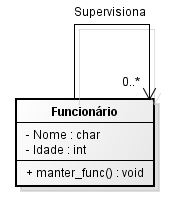
\includegraphics[scale=0.8]{imagens/associacao-unaria.jpg}
	\caption{Associação unária}
	\legend{Fonte: http://sgvclin.altervista.org/rea-uml/pop/pop-3/popup-texto3.html}
	\label{fig:associacao-unaria}
\end{figure}

Percebam que existe uma associação e próximo ao final da seta temos \textbf{0..*}. Esta informação representa a multiplicidade. A \textbf{multiplicidade} é extremamente semelhante a \textbf{cadinalidade} utilizada no Modelo Entidade-Relacionadal. Ela procura determinar qual das classes envolvidas em uma associação fornece informações para as outras, além de especificar o nível de dependências. 

\begin{figure}[H]
	\centering
	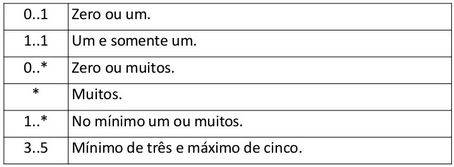
\includegraphics[scale=0.8]{imagens/multiplicidade.jpg}
	\caption{Multiplicidades}
	\legend{Fonte: http://sgvclin.altervista.org/rea-uml/pop/pop-3/popup-texto3.html}
	\label{fig:multiplicidades}
\end{figure}

\subsubsection{Associação binária} 

Uma associação binária ocorre quando são identificados relacionamentos entre duas classes. Este tipo de associação é o mais comum no diagrama de classe.

\begin{figure}[H]
	\centering
	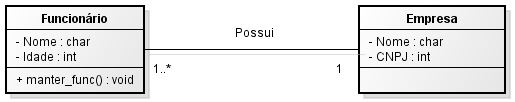
\includegraphics[scale=0.8]{imagens/associacaobinaria.jpg}
	\caption{Associação Binária}
	\legend{Fonte: http://sgvclin.altervista.org/rea-uml/pop/pop-3/popup-texto3.html}
	\label{fig:assbinaria}
\end{figure}

\subsubsection{Associação N-ária}

Já, uma associação N-ária, também conhecida como ternária, são aquelas mais de duas classes. Neste, além da linha associando as classes, também possuímos um losango para onde converge todas as ligações. 

\begin{figure}[H]
	\centering
	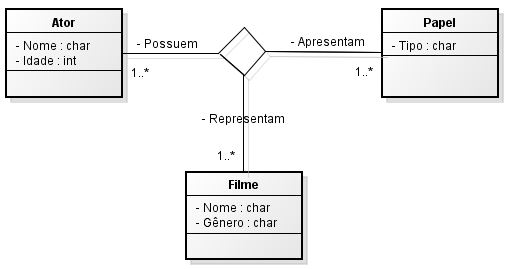
\includegraphics[scale=0.8]{imagens/associacao-ternaria.jpg}
	\caption{Associação N-ária}
	\legend{Fonte: http://sgvclin.altervista.org/rea-uml/pop/pop-3/popup-texto3.html}
	\label{fig:ass-enaria}
\end{figure}

\subsubsection{Agregação}

É um tipo especial de associação em que tenta-se demonstrar que as informações de um objeto (chamado objeto-todo) precisam ser complementados pelas informações contidas em um ou mais objetos de outra classe (chamados objetos-parte); conhecemos como todo/parte.

Esse tipo de associação é representada por um losango sem preenchimento no final da associação, sempre do lado do objeto \textbf{todo}.

\begin{figure}[H]
	\centering
	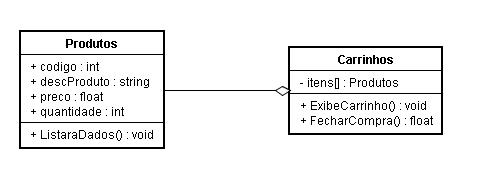
\includegraphics[scale=0.8]{imagens/agregacao2.jpg}
	\caption{Agregação}
	\legend{Fonte: http://www.cpscetec.com.br/adistancia/aula5.html}
	\label{fig:agregacao}
\end{figure}

\begin{figure}[H]
	\centering
	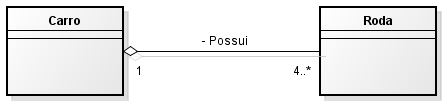
\includegraphics[scale=0.8]{imagens/7.JPG}
	\caption{Agregação}
	\legend{Fonte: http://sgvclin.altervista.org/rea-uml/pop/pop-3/popup-texto3.html}
	\label{fig:agregacao2}
\end{figure}

\subsubsection{Composição}

Pode-se dizer que composição é uma variação da agregação. Uma composição tenta representar também uma relação todo - parte. No entanto, na composição o objeto-pai (todo) é responsável por criar e destruir suas partes. Em uma composição um mesmo objeto-parte não pode se associar a mais de um objeto-pai.

\begin{figure}[H]
	\centering
	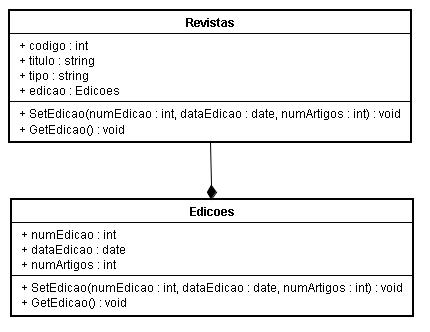
\includegraphics[scale=0.8]{imagens/DC_Composicao.jpg}
	\caption{Composição}
	\legend{Fonte: http://www.cpscetec.com.br/adistancia/aula5.html}
	\label{fig:composicao1}
\end{figure}

\begin{figure}[H]
	\centering
	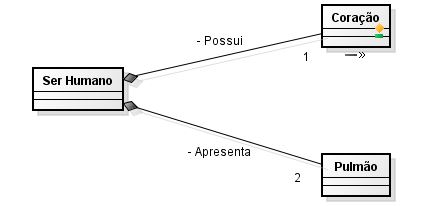
\includegraphics[scale=0.8]{imagens/8.JPG}
	\caption{Composição}
	\legend{Fonte: http://sgvclin.altervista.org/rea-uml/pop/pop-3/popup-texto3.html}
	\label{fig:composicao2}
\end{figure}

\subsubsection{Especialização/Generalização}

Especialização/Generalização ou também chamada de Herança. Este tipo de associação ocorre quando uma classe gera novas classes que sejam suas cópias perfeitas e a partir destas classes é possível adaptá-las ao meio em que sejam necessárias. A classe que é usada como referência é conhecida por \textbf{superclasse / generalização} ou classe mãe, a classe criada com base nessa superclasse é conhecida como \textbf{sub-classe / especialização} ou classe filha. Na classe filha, podemos redefinir métodos e criar novos campos.

\begin{figure}[H]
	\centering
	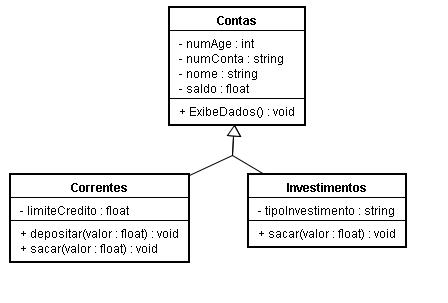
\includegraphics[scale=0.8]{imagens/heranca.jpg}
	\caption{Especialização/Generalização}
	\legend{Fonte: http://www.cpscetec.com.br/adistancia/aula5.html}
	\label{fig:composicao1}
\end{figure}

\begin{figure}[H]
	\centering
	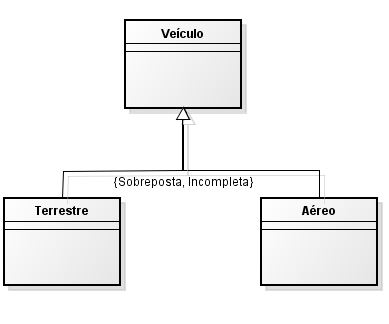
\includegraphics[scale=0.8]{imagens/9.JPG}
	\caption{Especialização/Generalização}
	\legend{Fonte: http://sgvclin.altervista.org/rea-uml/pop/pop-3/popup-texto3.html}
	\label{fig:composicao2}
\end{figure}

\subsection{Encapsulamento}

Conceitua-se encapsulamento como sendo o processo utilizado para proteger os campos e operações de uma classe (atributos e métodos), permitindo que apenas os membros públicos sejam acessados pelos usuários de determinada classe.

Para atingir o encapsulamento, uma das formas é definindo a visibilidade das propriedades e dos métodos de um objeto. A visibilidade define a forma como essas propriedades devem ser acessadas.

\begin{table}[H]
	\resizebox{\textwidth}{!}{%
		\begin{tabular}{|l|l|}
			\hline
			\textbf{Público - public} & \begin{tabular}[c]{@{}l@{}}Nível de acesso livre. Indica que o método ou atributo da classe é público, \\ ou seja, pode-se acessar este atributo, ou executar esse método, por qualquer código de programa. \\ Usamos o sinal (+) na notação UML para simbolizar essa visibilidade.\end{tabular} \\ \hline
			\textbf{Privado - private} & \begin{tabular}[c]{@{}l@{}}Nível mais protegido. Mebros declarados como private, só podem ser acessados dentro \\ da classe em que foram declarados. Usamos o sinal (-) na notação UML para simbolizar essa \\ visibilidade.\end{tabular} \\ \hline
			\textbf{Protegido - protected} & \begin{tabular}[c]{@{}l@{}}Nível de acesso intermediário. Serve para que o método ou o atributo seja público dentro \\ do código da própria classe e de qualquer classe que herde daquela onde está o método ou \\ propriedade protected. É privado e não acessível de qualquer outra parte. Usamos o sinal (\#) \\ na notação UML para simbolizar essa visibilidade.\end{tabular} \\ \hline
		\end{tabular}%
	}
\end{table}

\begin{figure}[H]
	\centering
	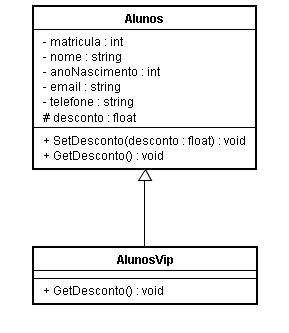
\includegraphics[scale=0.8]{imagens/DC_vip.jpg}
	\caption{Encapsulamento}
	\legend{Fonte: http://www.cpscetec.com.br/adistancia/aula5.html}
	\label{fig:encapsulamento}
\end{figure}

\subsection{Exercícios de fixação}

\begin{enumerate}
	\item Uma empresa possui fornecedores de peças. Aos fornecedores é atribuído um código que os identifica univocamente. O mesmo procedimento é usado para as peças. Os fornecedores possuem ainda um nome, endereço e telefone. As peças são caracterizadas por designação e cor. As cores podem ser preto, branco, cinzento e vermelho. Os fornecimentos são feitos a um dado preço e numa dada data.
	\item Cada escola da comunidade Alfa é dividida em um ou mais departamentos (letras, matemática, etc.). Um departamento é chefiado por um de seus professores, mas há casos em que esse cargo está vago. Não há acúmulo de chefia. Professores podem estar alocados em um ou mais departamentos. Um departamento pode ser criado sem que haja professores a ele alocados. Um aluno pode estar matriculado em mais de uma escola e pode frequentar mais de um curso na mesma escola. Escolas podem não ter alunos matriculados. Cada departamento tem seu conjunto específico de cursos (pelo menos um). Cada curso pode ser ministrado por um ou mais professores. Cada professor pode ministrar qualquer número de cursos.
	\item Para cada obra armazena-se o ISBN, o(s) autor(es), o título, a editora, o assunto e a edição. Os exemplares possuem a data de inclusão no acervo e uma marcação de disponibilidade (as bibliotecas só cadastram obras que constam do acervo).
	As bibliotecas emprestam livros aos alunos e aos membros da comunidade. Alunos podem retirar até 2 títulos; membros da comunidade podem retirar apenas um título por vez.
	\item Uma empresa efetua encomendas, numeradas. Cada encomenda possui um número variável de itens, cada um das quais diz respeito a um produto a ser encomendado. Os itens possuem uma ordem numérica dentro de cada encomenda. A encomenda tem uma data e dirige-se a um só fornecedor. Tanto os produtos como os fornecedores são identificados por um código próprio. Os itens incluem o número dom item, o código do produto, o preço unitário e a quantidade encomendada.
\end{enumerate}